\section{Kartoteket - Daniel Rapp}
\subsection{Inledning}
Idag är information om Region Östergötlands operationsartiklar, så som priserna och
placeringen i lagret på tandborstar, tandkräm, handskar och annan
medicinsk utrustning, hanterat av ett internt system.
Detta system kallas ett "\textit{kartotek}", och är helt enkelt en sorts artikeldatabas.
I vårt system så ska detta uppdateras och förbättras på olika sätt.

\subsubsection{Syfte}
Syftet med denna del är att beskriva vad kartoteket är samt
hur vår förbättrade lösning är uppbyggd.


\subsubsection{Frågeställning}
Frågeställningar:
\begin{itemize}
  %\item Kan man implementera ett kartotekssystem som uppfyller kundens önskemål?
  %\item Går det att implementera ett kartotekssystem som 
  \item Går det att integrera systemet för handböcker med kartoteket utan att förlora funktionalitet?
\end{itemize}


\subsubsection{Avgränsningar}
Förutom ett förbättrat kartotekssystem så är Region Östergötland också i behov av
ett bättre system för att hantera deras lager på ett mer automatiserat sätt.
Bland annat så skulle de behöva ett system som låter dem checka in vilka varor från lagret de hämtat
ut, istället för att checka av manuellt, vilket kan vara felbenäget.

Vi valde dock att avgränsa oss från att bygga denna lösning, på grund av tidsbrist.
Istället fokuserade vi på att förbättra kärnfunktionaliteten i applikationen.


\clearpage
\subsection{Bakgrund}
I dagsläget använder Region Östergötland sig av två separata system
för att förbereda operationer. En handbok (se ovan) och ett kartotek (se figur \ref{fig:kartotek}).
Dessa är för tillfället helt separata applikationer.

\begin{figure}[h!]
  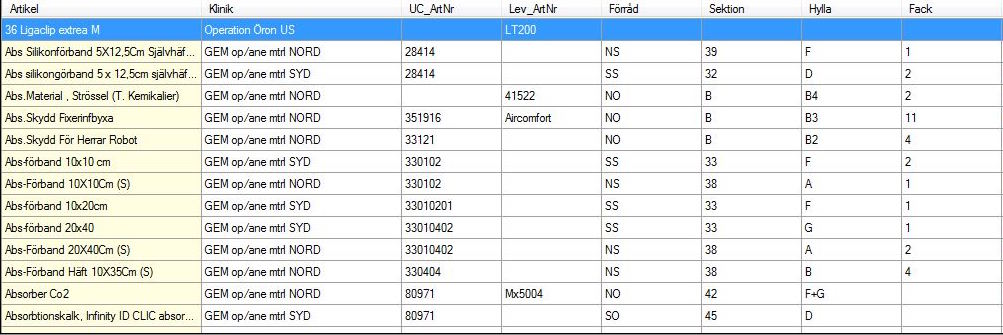
\includegraphics[width=0.9\textwidth]{../images/forradsinfo.jpg}
  \caption{Gamla kartoteket}
  \label{fig:kartotek}
\end{figure}

Så om en artikel har utgått eller Region Östergötland
väljer att inte köpa in en viss artikel längre så tar de bort artikeln
från kartoteket. Problemet som då uppstår är att detta inte reflekteras
i handböckerna. Så om t.ex. en "\textit{Oral-B Pro 600 CrossAction}"\ tandborste används i
en "\textit{Laparoskopisk sigmoideumresektion}", och tandborsten utgår
så tas den bort från kartoteket, men eftersom handboken för operationen inte är
kopplad till kartoteket så uppdateras det inte att denna artikel inte längre finns i lagret.

Vår förbättrade lösning
integrerar systemet som hanterar handböcker tillsammans med ett nytt kartotek,
där allt är byggt på webben. När en artikel ändras eller tas bort i kartoteket
så ändras den även i alla handböcker för operationer som kräver denna artikel.



%\subsection{Teori}
\subsection{Metod}
Precis som resten av systemet så är kartoteket skrivet på webben, och
därmed i javascript, HTML och CSS.
Vi har även använt Git för versionshantering.

Jag måste också nämna att trots att det är jag som skriver om kartoteket,
så är det inte endast jag som har implementerat det. Koden och gränssnittet har givetvis
varit ett stort grupparbete mellan alla medlemmar.


\clearpage
\subsection{Resultat}
Resultatet av vårt arbete är ett förbättrat kartotekssystem
som integrerar data från handboken till ett uniformt system.

Kärnfunktionaliteten i kartoteket är möjligheten att se, modifiera och hitta artiklar.
Så resultatet kommer presenteras i tre delar.

\subsubsection{Att se artiklarna}
När man först kommer in på sidan för att hantera kartoteket så
blir man välkomnad av en stor tabell som innehåller alla artiklar
i kartoteket (runt 3000 för tillfället). Se figur \ref{fig:table}.

\begin{figure}[h!]
  \centering
  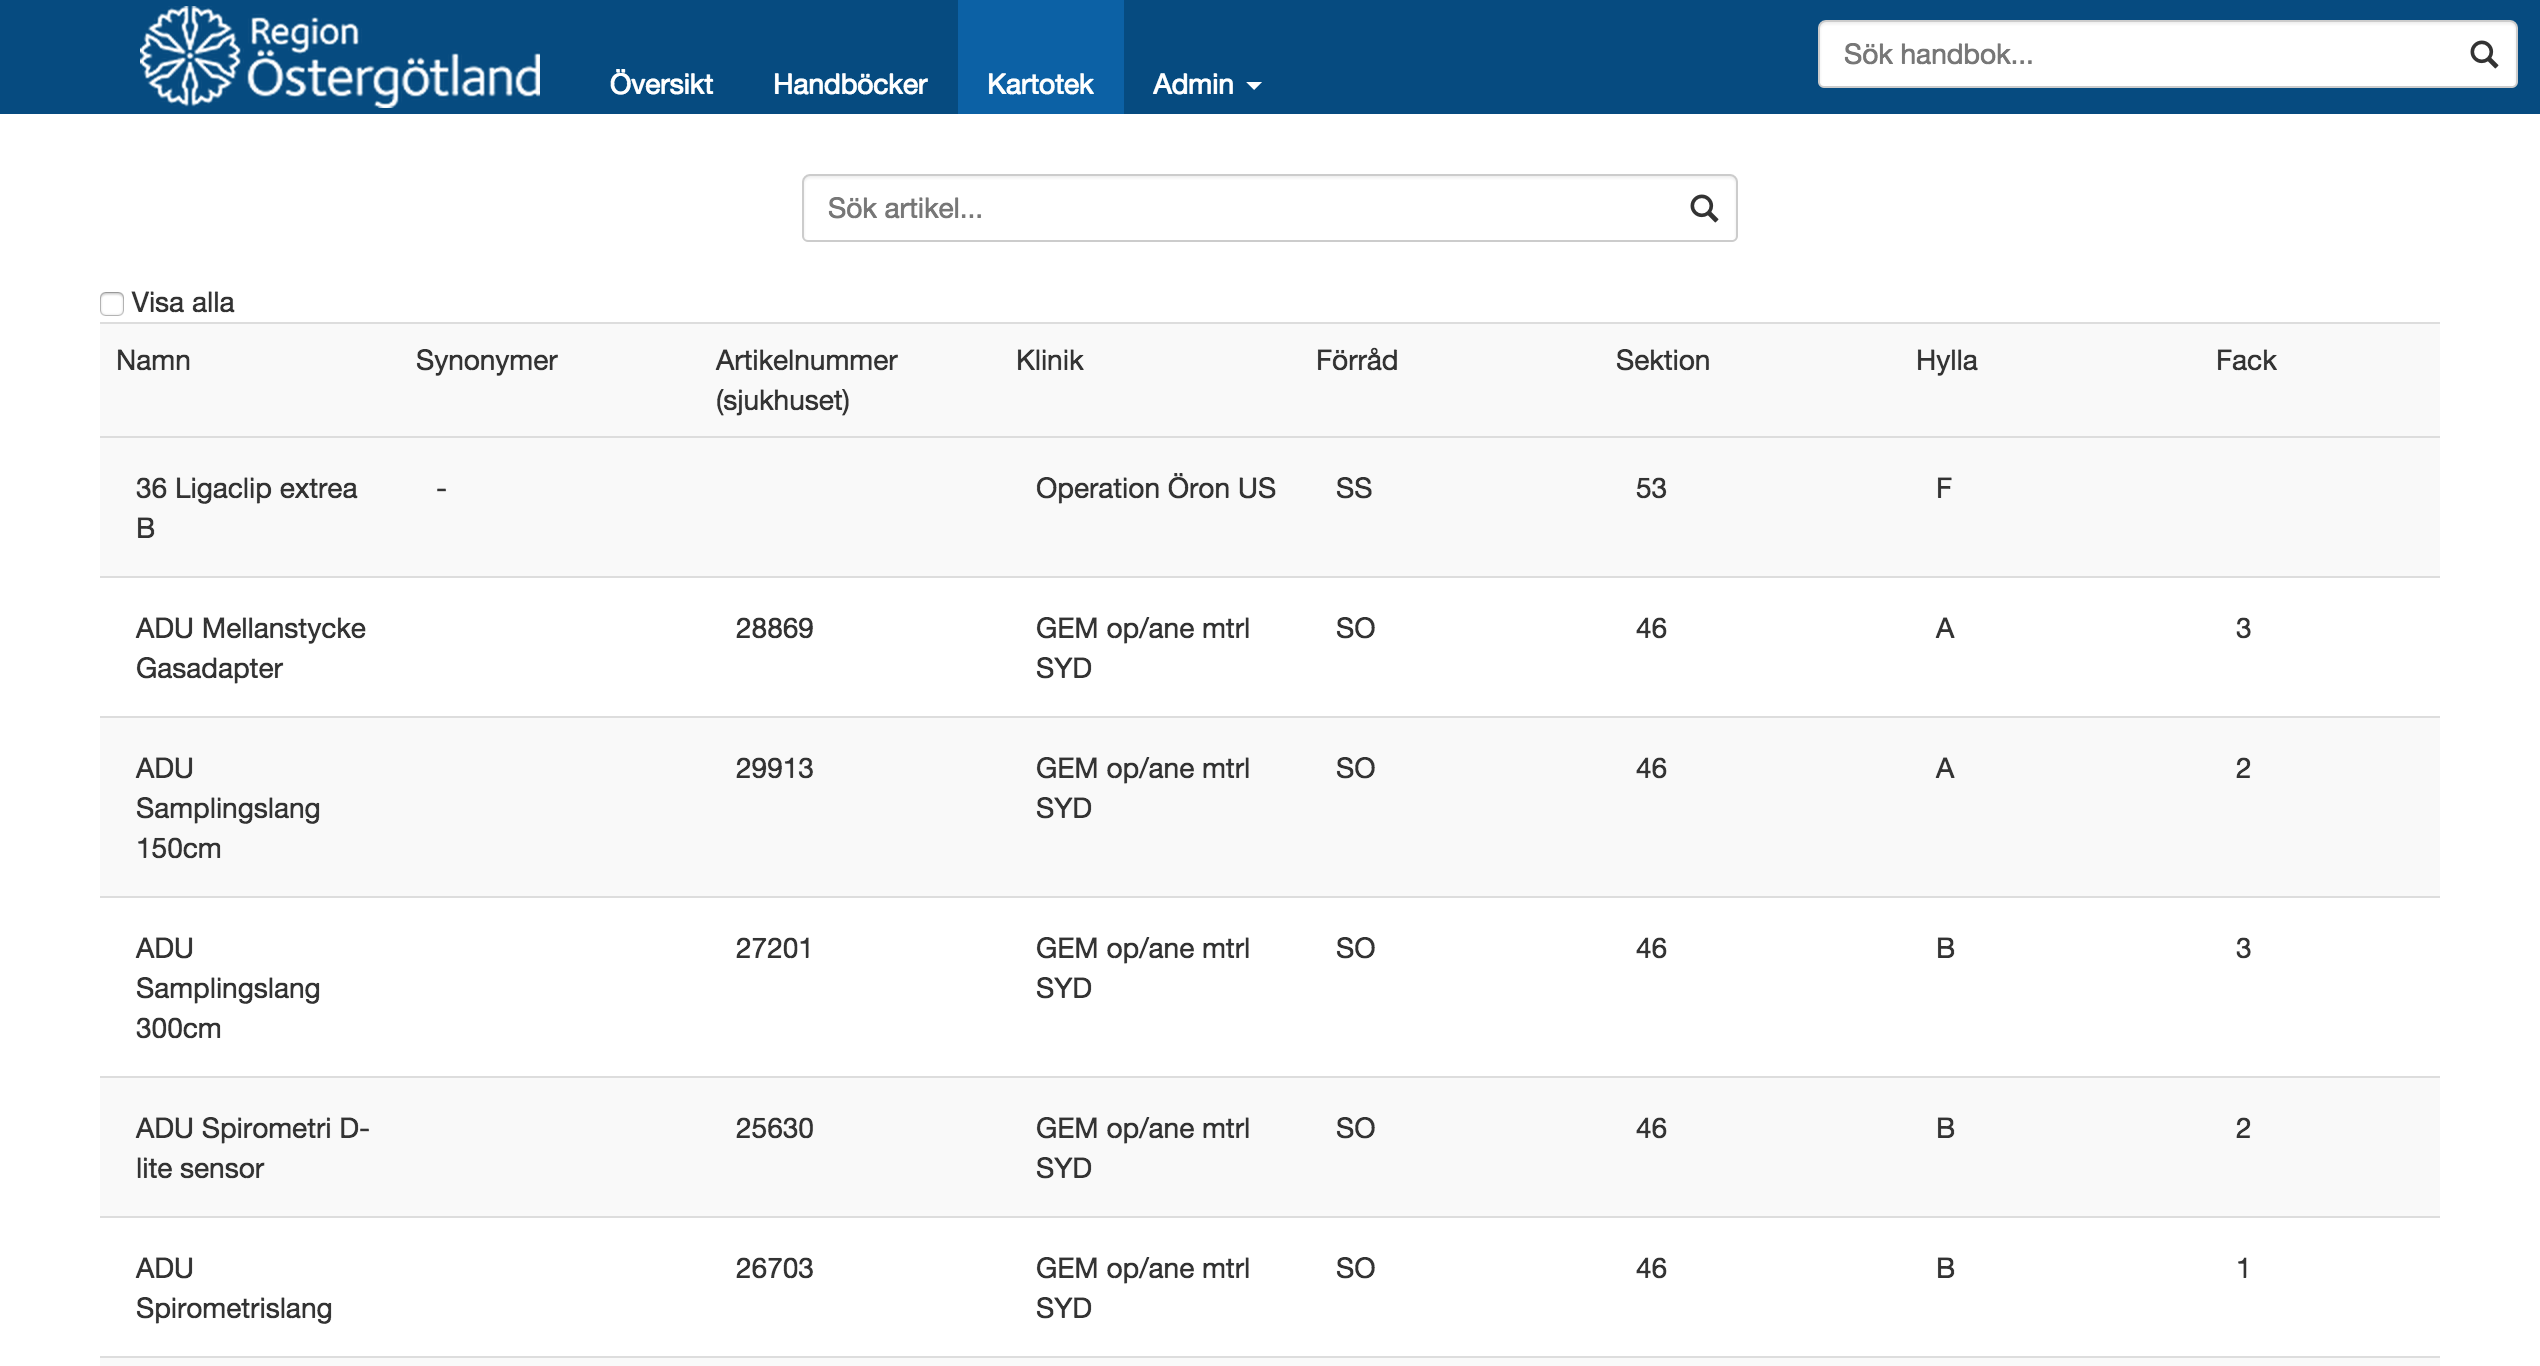
\includegraphics[width=0.9\textwidth]{../images/kartotek1.png}
  \caption{Kartoteket}
  \label{fig:table}
\end{figure}

Först laddas endast runt 50 artiklar, men
om man skrollar ner så laddas fler.

Det finns två olika sätt att se informationen.
Två olika vyer.

Den ena är standardvyen, som man ser om man inte är inloggad
eller inte är administratör. Denna vyn kan ses i figur \ref{fig:table}
och innehåller endast den mest nödvändiga informationen om
artiklarna, som namn, klinik, förråd, etc.

Den andra vyn är administratörsvyn.
Man kommer endast in på denna vy om man är administratör.
Om man aktiverar denna så utvidgas tabellen för att
visa mer information om artiklarna, bland annat pris på artiklarna.
Vi har valt att inte inkludera en bild på denna information
då detta är sekretessbelagt.

I den här vyn finns också möjligheten att ta bort, lägga till och modifiera
information om artiklar, vilket är vad de två följande delarna handlar om.

\clearpage
\subsubsection{Modifiering av artiklarna}
För att modifiera artiklar så måste man som sagt vara administratör.

Med vårt gränssnitt så är det enkelt att modifiera information om en artikel.
Om man vill ändra på, t.ex., artikelnamnet så är det bara att klicka på det!
En input-ruta kommer då upp som låter dig ändra namnet till någonting mer passande.
Detta är inspirerat av Trello, som vi använder för att organisera saker att göra.
I Trello så finns en liknande funktionalitet för att ändra namn på olika "\textit{Boards}".

För att ta bort artiklar så finns det ett smidig "X" till vänster om artikel-raden.

Vi har valt att göra en del av den här informationen obligatorisk, eftersom
sjukhuset hade problem i sitt tidigare system att vissa sjuksköterskor skippade
att skriva in en del viktig information om artikeln.


\subsubsection{Sökning av artiklarna}
Sista kärnfunktionaliteten i kartoteket är sökning.
Eftersom artiklarna är sorterade i bokstavsordning,
och kartoteket har en "infinite scroll"-funktionalitet,
så går det i teorin att hitta alla artiklar utan att söka.
I våra diskussioner kunden på sjukhuset så
verkar det också som det finns vissa personer som primärt använder
sig av denna metod för att hitta artiklar.
Däremot är detta inte en speciellt effektiv lösning, så därför
har vi valt att implementera en sökfunktion.

\begin{figure}[h!]
  \centering
  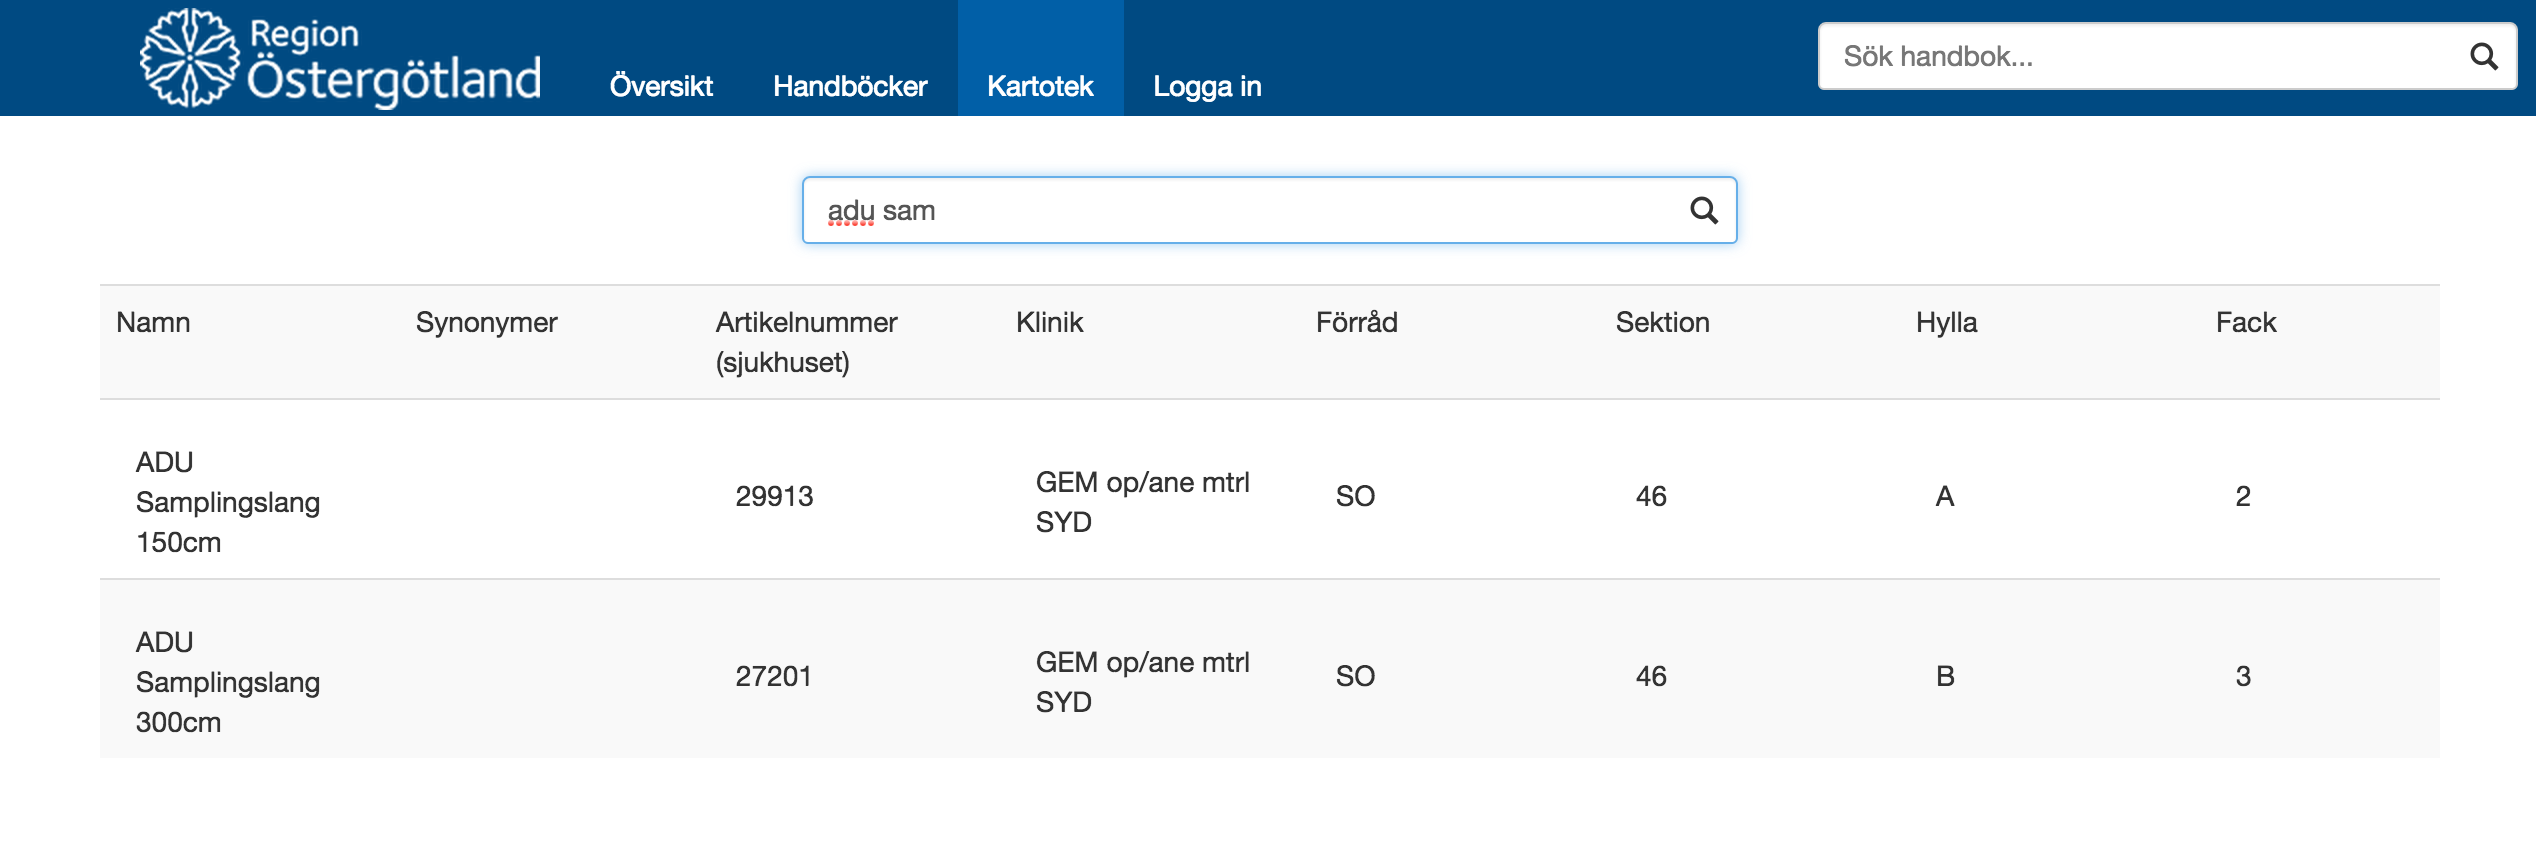
\includegraphics[width=0.9\textwidth]{images/site/kartsearch.png}
  \caption{Sökning i kartoteket.}
  \label{fig:kartsearch}
\end{figure}

Sökfunktionen är enkel.
Längst upp på sidan finns det en liten sökruta.
Användaren har möjlighet att söka på artikelnamn, artikelnummer
eller synonymer till namnet. Se ett exempel på sökning
av artikelnamn i figur \ref{fig:kartsearch}.
När man söker på någonting så byts hela tabellen ut mot sökresultatet.
Hela upplevelsen är inspirerat av "\textit{Google Instant}".

\clearpage
\subsubsection{Integrering med handböckerna}
Kartoteket står inte i isolation.
En nyckelanledning till att det är så användbart är
för att det är integrerat med handböckerna.
Det leder oss till frågeställningen:
\begin{quote}
  Går det att integrera systemet för handböcker med kartoteket utan att förlora funktionalitet?
\end{quote}
Svaret på detta anser jag vara: Ja!
Och i detta avsnitt hade jag tänkt övertyga om denna slutsats.

Integreringen sker primärt på två ställen.
\begin{enumerate}
  \item När man skapar en ny handbok.
  \item När man förbereder en operation.
\end{enumerate}

När man skapar en handbok så är kartoteket integrerat på det sättet att
när man lägger till artiklar som måste hämtas från lagret så söker man
i kartoteket för att hitta dessa. Detta är en förbättring av förra
systemet då det förut inte fanns det ingen koppling mellan dessa system.

När man förbereder en operation så är kartoteket integrerat på
så sätt att om en artikel slutar säljas, eller den av någon anledning
tas bort från kartoteket, informerar vi användaren om att den
har utgått.

Som vi har nämnt tidigare så fanns ingen av dessa av dessa funktionaliteter
förut. Eftersom vi dessutom har lyckats reproducera all funktionalitet
som fanns i det förra systemet så anser jag att frågan är klart och
tydligt positivt bekräftad.


\subsection{Diskussion}
Har vi lyckats med kartoteket? Och framför allt, är
kunden nöjd? Fick kunden de dom önskade?

Svaret är otvivelaktigt: Ja! Det finns
givetvis små buggar här och där. Ingen
produkt blir någonsin 100\% bugg-fri.
Men i våra informella intervjuer under de två studiebesök vi gjorde hos kunden
under iteration 3, där kunden har testat
vårt system en hel dag, så verkade de enormt nöjda.


%\subsubsection{Resultat}
%\subsubsection{Metod}


\subsection{Slutsatser}
Allt som allt så blev vi väldigt nöjda med kartoteket.
Det finns såklart, som alltid, saker vi skulle vilja förbättra om vi
hade mer tid, som integrering i lagret med t.ex. saldo.
Men vi anser det som finns nu, kärnfunktionaliteten,
ger en märkbar förbättring gentemot det nuvarande systemet.




\subsection{Referenser}
\vspace{-9mm}
\begin{thebibliography}{9}

\end{thebibliography}
